\documentclass[12pt,a4paper]{article}
\usepackage{Preamble}
\usepackage{subfiles}

\begin{document}
\maketitle
\tableofcontents

\section{Introduction}
Good circuit design is more than simply calculating the “correct” component values, it is ensuring that the circuit behaves properly when it has been manufactured in large quantities! Part of that evaluation is ensuring that the circuit performs adequately within the bounds of production tolerances. Student projects, by their nature, are often one-off designs, and students have the ability to adjust component values to account for outputs that are not quite what was expected. In a production setting, this is not a feasible strategy.

This project will produce a front-end for the Spice circuit simulator that supports the testing of designs across the range of possible production values of components. The input to the simulator will be a Spice simulation file (previously tested using a package such as LTSpice), and a set of component tolerances. The project will then proceed to run the simulation multiple times, for the different component tolerances, to test out the impact of these on the final output.

\section{Installation}
\begin{itemize}
    \item \textbf{Requirement}\par
    ngspice = 34\par
    python3\par
    Module: numpy, scipy, PyQt5 $\geqslant$ 5.15, matplotlib, pandas, django, quantiphy\par
    Optional Module: bs4, weasyprint, coloredlogs\par

    \item  \textbf{Ngspice Configuration}\par
    Ngspice should be installed in directory \textit{./Workspace}. It can be downloaded from \href{https://sourceforge.net/projects/ngspice/}{sourceforge ngspice Git page}.

    To compile ngspice34, make sure you enable the relative paths for spinit and code models.
    \lstset{backgroundcolor=\color{white},numbers=none,keepspaces=false}
    \begin{lstlisting}
    $ ./configure --enable-relpath
    \end{lstlisting}

    The normal compile command for linux-64 bit installed is
    \begin{lstlisting}{language=bash}
    $ ./configure --with-x --enable-xspice --enable-cider --with-readline=yes --enable-openmp --enable-relpath --prefix={PATH-TO-Workspace} --disable-debug CFLAGS="-m64 -O2" LDFLAGS="-m64 -s"
    \end{lstlisting}
    Where PATH-TO-Workspace is the complete path to the dirctory \textit{Workspace}
\end{itemize}

\section{Block Diagram}
\begin{figure}[ht]
    \centering
    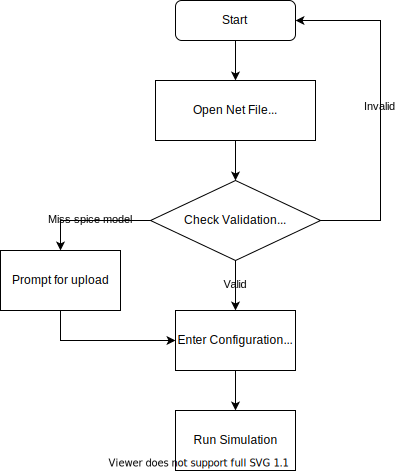
\includegraphics[width=0.75\textwidth]{Image/spice.pdf}
    \caption{}
\end{figure}

\section{Project structure}
This project is mainly written in python3 and for circuit analysis part, it is written in spice language.

\subsection{main.py}
Main function of the project.

\noindent\textbf{Variable Description}
\begin{itemize}
    \item \textcolor{blue}{root}: Root path of main.python3
    \item \textcolor{blue}{path}: PATH variable of the system
\end{itemize}

\subsection{src/read.py}
Read in a circuit file

\begin{itemize}[leftmargin=*]
    \item \textcolor{blue}{rm(*filename)}\\
        Delete the given files. If the file does not exist, pass.

    \item Class \textcolor{blue}{C}\\
        Capacitor.\\
        \textbf{Attribute:}
        \begin{itemize}
            \item \textcolor{blue}{C.name}: Capacitor name
            \item \textcolor{blue}{C.c}: Capacitance value
            \item \textcolor{blue}{C.tol}: Capacitor tolerance
        \end{itemize}

    \item Class \textcolor{blue}{R}\\
        Capacitor.\\
        \textbf{Attribute:}
        \begin{itemize}
            \item \textcolor{blue}{R.name}: Resistor name
            \item \textcolor{blue}{R.r}: Resistance value
            \item \textcolor{blue}{R.tol}: Resistor tolerance
        \end{itemize}

    \item Class \textcolor{blue}{circuit}\\
        Circuit class.\\
        \textbf{Attribute:}
        \begin{itemize}
            \item Initialize\\
                Give the file name of the netlist file.
            \item \textcolor{blue}{circuit.read()}\\
                Read in the netlist.

                Accpetable control command in netlist: ".model", ".subckt", ".global", ".include", ".lib", ".temp", ".ends", ".ac", ".probe"

                \textbf{Caution:} All commands between \textbf{.control} and \textbf{.endc} will be ignored.
            \item \textcolor{blue}{circuit.init()}\\
                Initialize the circuit, check if any error in circuit file.

                It will call the ngspice to first perform an operating point analysis. During this process, it will give us all the component and net information.

                If the operation point analysis is passed, it will perform an AC, small-signal frequency response
                analysis.

                \textbf{Return:} two-element tuple(error\textunderscore message, flag).

                flag=0: no error occurs or uncategorized error

                flag=1: include file error. Could not find include file

                flag=2: Unknown subcircuit error.

                If no error occur, both elements are 0.

            \item \textcolor{blue}{circuit.fixinclude(self, repl, mode)}\\
                Fix the error, missing the include file or subcircuit file.

                \textbf{Parameters:}\\
                repl: uploaded include file\\
                mode: 1 or 2. 1 represents include file error, 2 represents subcircuit error.

            \item \textcolor{blue}{circuit.readnet()}

\end{itemize}

\subsection{src/\textunderscore write.py}
Write control files. This is the subfile for class \textcolor{blue}{circuit}, defining new attributes.

\begin{itemize}[leftmargin=*]
    \item \textcolor{blue}{circuit.create\textunderscore prerun()}\\
        Create the control file \textit{run\textunderscore control \textunderscore pre.sp}. It tests the circuit before the formal simulation. Measuring max and min gain does not require this function to run.

    \item \textcolor{blue}{circuit.create\textunderscore sp(add=False)}\\
        Create the main simulation control file \textit{run\textunderscore control.sp}

    \item \textcolor{blue}{circuit.create\textunderscore wst()}\\
        Create the control file \textit{run\textunderscore control\textunderscore wst.sp} for the worst case simulation.

    \item \textcolor{blue}{circuit.create\textunderscore step()}\\
        Create the control file \textit{run\textunderscore control.sp} for the step mode.

    \item \textcolor{blue}{circuit.create\textunderscore opamp()}\\
        Create the control file \textit{run\textunderscore control.sp} for switching op amp.

    \item \textcolor{blue}{circuit.create\textunderscore cmrr(add=False)}\\
        Create the control file \textit{run\textunderscore control.sp} and \textit{run\textunderscore control\textunderscore wst.sp} for CMRR mode.

        If add=True, control file \textit{run\textunderscore control\textunderscore wst.sp} will not be created as it would have been run when first created.

\end{itemize}

\subsection{src/\textunderscore resultaly.py}
Analyse simulation results and create report. This is the subfile for class \textcolor{blue}{circuit}, defining new attributes.

\begin{itemize}
    \item \textcolor{blue}{circuit.resultdata(self, worst=False, add=False, mode=None)}\\
        Analyse simulation results.

        Parameters:

        worst: Bool, Optional\par
        \quad If true, it will analyse the worst case simulation data.

        add: Bool, Optional\par
        \quad If true, this function read in data from last end read point.

        mode: Str, Optional\par
        \quad This function would analyse data using importance sampling by default.

        \quad Available choice: 'Opamp' and 'Step'

    \item \textcolor{blue}{f(x, miu, sigma, tol)}\\
        Importance sampling function. It calculates:
        \begin{equation*}
            \frac{\exp\left [\frac{(x-\mu)^2}{2\sigma^2}\right ]}{\frac{\text{erf}(\frac{tol\cdot\mu}{\sqrt{2}\sigma\pi})-\text{erf}(\frac{tol\cdot\mu}{\sqrt{2}\sigma\pi})}{2}\sigma\sqrt{2\pi}}
        \end{equation*}

    \item \textcolor{blue}{circuit.report(mode=None)}\\
        Generate html5 report.
\end{itemize}

\subsection{src/plot.py}
Code for GUI interface.

\textbf{Class \textcolor{blue}{plotGUI(QtWidgets.QMainWindow)}}

Main GUI interface.

\begin{itemize}
    \item UI file: main.ui\par
        To edit this file, you can install module qt5-applications by
        \lstset{backgroundcolor=\color{white},numbers=none,keepspaces=false}
        \begin{lstlisting}
        pip install qt5-applications
        \end{lstlisting}

        Open the designer in Path-to-site-packages/qt5\textunderscore applications/Qt/bin/designer and edit it.
        \begin{figure}[ht]
            \centering
            \includegraphics[width=0.9\textwidth]{Image/main.eps}
            \caption{}
        \end{figure}


    \item \textcolor{blue}{openfile()}\\
        Open a new netlist file. If there is a new opened, warn the user with a message box.

        It will first copy the selected file to a new folder, named with the filename and uploaded time. Then, call the function to read the file. If no error occur, call the function to initialzie the circuit. If some error happens, it will pop out a window. Finally, show the configuration window.

    \item \textcolor{blue}{configCreate()}\\
        Read in parameters from configuration window. Check the validity of the parameters and call specific function to create control files.

    \item \textcolor{blue}{configreject()}\\
        If 'cancel' is clicked in the configuration window, this function will run if the signal is connected to this function.

    \item \textcolor{blue}{start\textunderscore process(finishmode, runmode=0)}\\
        Call ngspice to do simulation.

        Parameters:

        \quad finishmode: String, Required

        \quad Available options:

        \quad runmode: int, optional

        \quad runmode=0, run only run\textunderscore control.sp

        \quad runmode=1, run both run\textunderscore control.sp and run\textunderscore control\textunderscore wst.sp

    \item \textcolor{blue}{kill()}\\
        Kill the ngspice if \textit{Cancel} is clicked while it is running.

    \item \textcolor{blue}{finishrun(mode)}\\
        This function will run when ngspice simulation is finished.

        mode: String, Required. It determines which method the result data would be processed.

    \item \textcolor{blue}{postinit(mode=None)}\\
        Do some post-initialization after running simulation.

    \item \textcolor{blue}{plot(mode=None)}\\
        Plot the data on the main window.

    \item \textcolor{blue}{plotwst()}\\
        Plot the worst case data.

    \item \textcolor{blue}{AddTime()}\\
        Add more simulation time.

    \item \textcolor{blue}{calcp()}\\
        Calculate the y axis value.

    \item \textcolor{blue}{analy()}\\
        If the button analysis is clicked.

    \item \textcolor{blue}{reset()}\\
        If the reset button is clicked.

\end{itemize}

\subsection{src/\textunderscore subwindow.py}
Define the Processing window and configuration window.

\begin{figure}[ht]
    \centering
    \includegraphics[width=0.9\textwidth]{Image/config.eps}
    \caption{Configuration window simulation tab}
\end{figure}

\begin{figure}[ht]
    \centering
    \includegraphics[width=0.9\textwidth]{Image/config34.eps}
    \caption{Configuration window CMRR and Op amp tab}
\end{figure}

\subsection{src/MplWidget.py}
The header file for the plotting area of both configuration window and main window.

\subsection{src/Logging.py}
Log file definition and some initialization of the tool.

\end{itemize}


\section{GUI Guide}
\subsection{Main Window}

\subsection{Configuration Window}

\subsection{Report}
To see html5 report, under the directory src/report, run the below command.
\lstset{backgroundcolor=\color{white},numbers=none,keepspaces=false}
\begin{lstlisting}
    python3 -m manage.py runserver
\end{lstlisting}

Then open 127.0.0.1:8000, you can see the result report.

Or you can find the html5 code file under src/htmlreport/templates/report.html

If you have the module weasyprint installed, you can find the pdf report under the circuit file base directory in folder Workspace.


\bibliographystyle{agsm}
%\bibliography{}

\end{document}